\section{Resultados}

Al realizar un Porkchop plot con la data obtenida de la tabla 1
\parencite{xia2021}, obtuvimos el siguiente resultado:

\begin{center}
    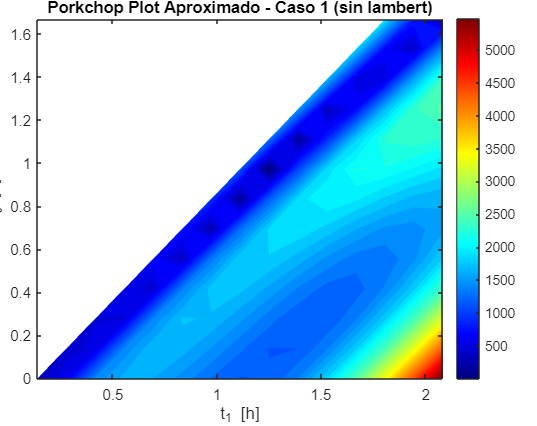
\includegraphics[width=0.4\textwidth]{porkchop_emma.jpg}
    \captionof{figure}{Porkchop resultante}
\end{center}

Las franjas azules indican mínimos, los cuales muestran una posible ventana de
impulso para interceptar a los dos objetos.